\section{Sequence diagrams}
\begin{figure}[!ht]
	\centering
	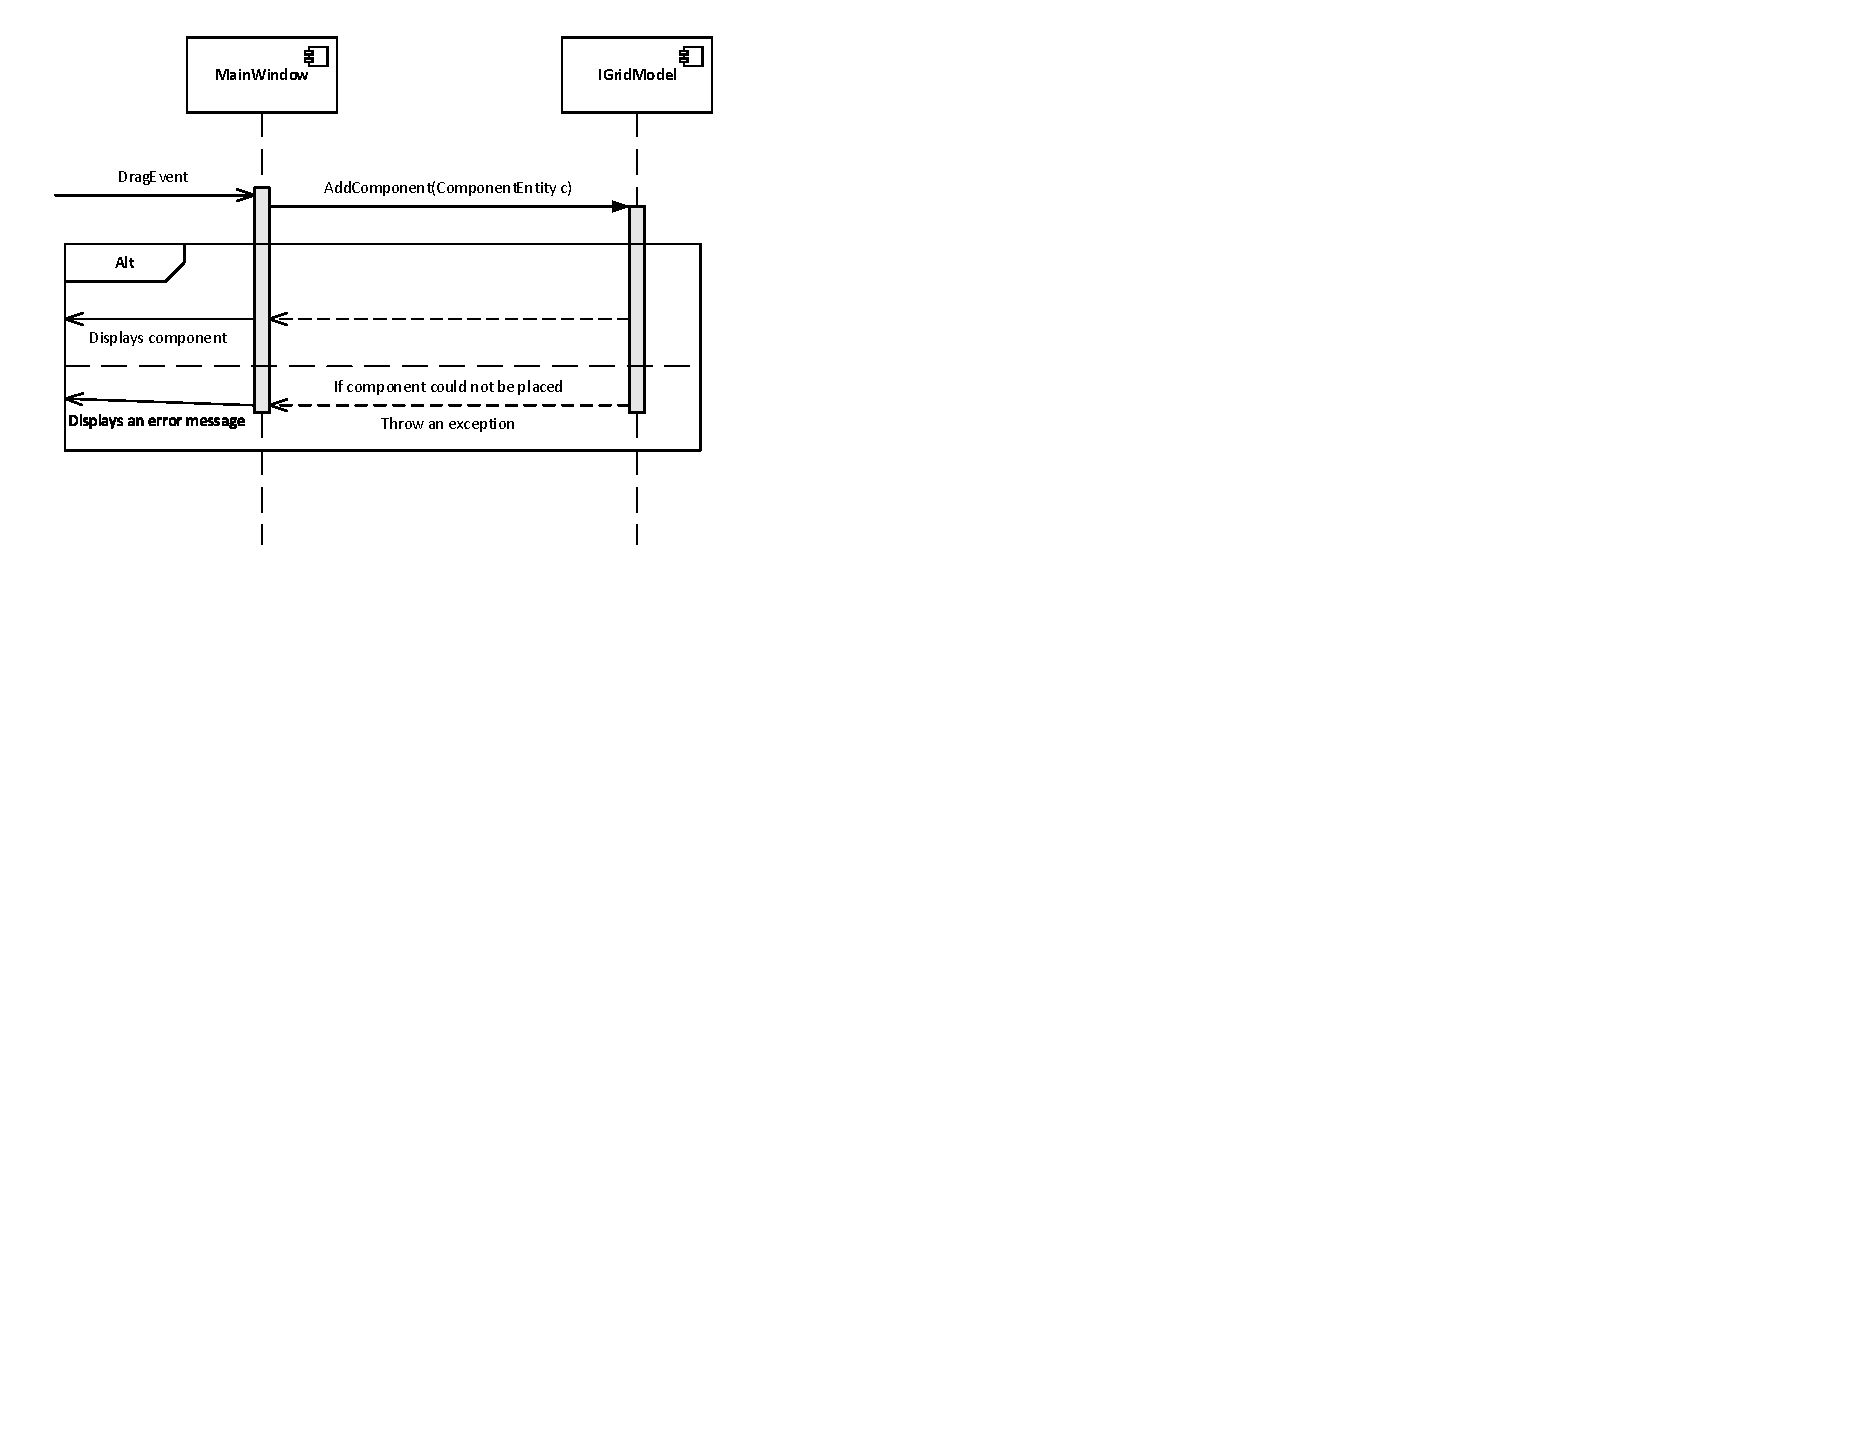
\includegraphics{figures/PosititioningCrossroad}
	\caption{Positioning crossroad.}
\end{figure}

\begin{figure}[!ht]
	\centering
	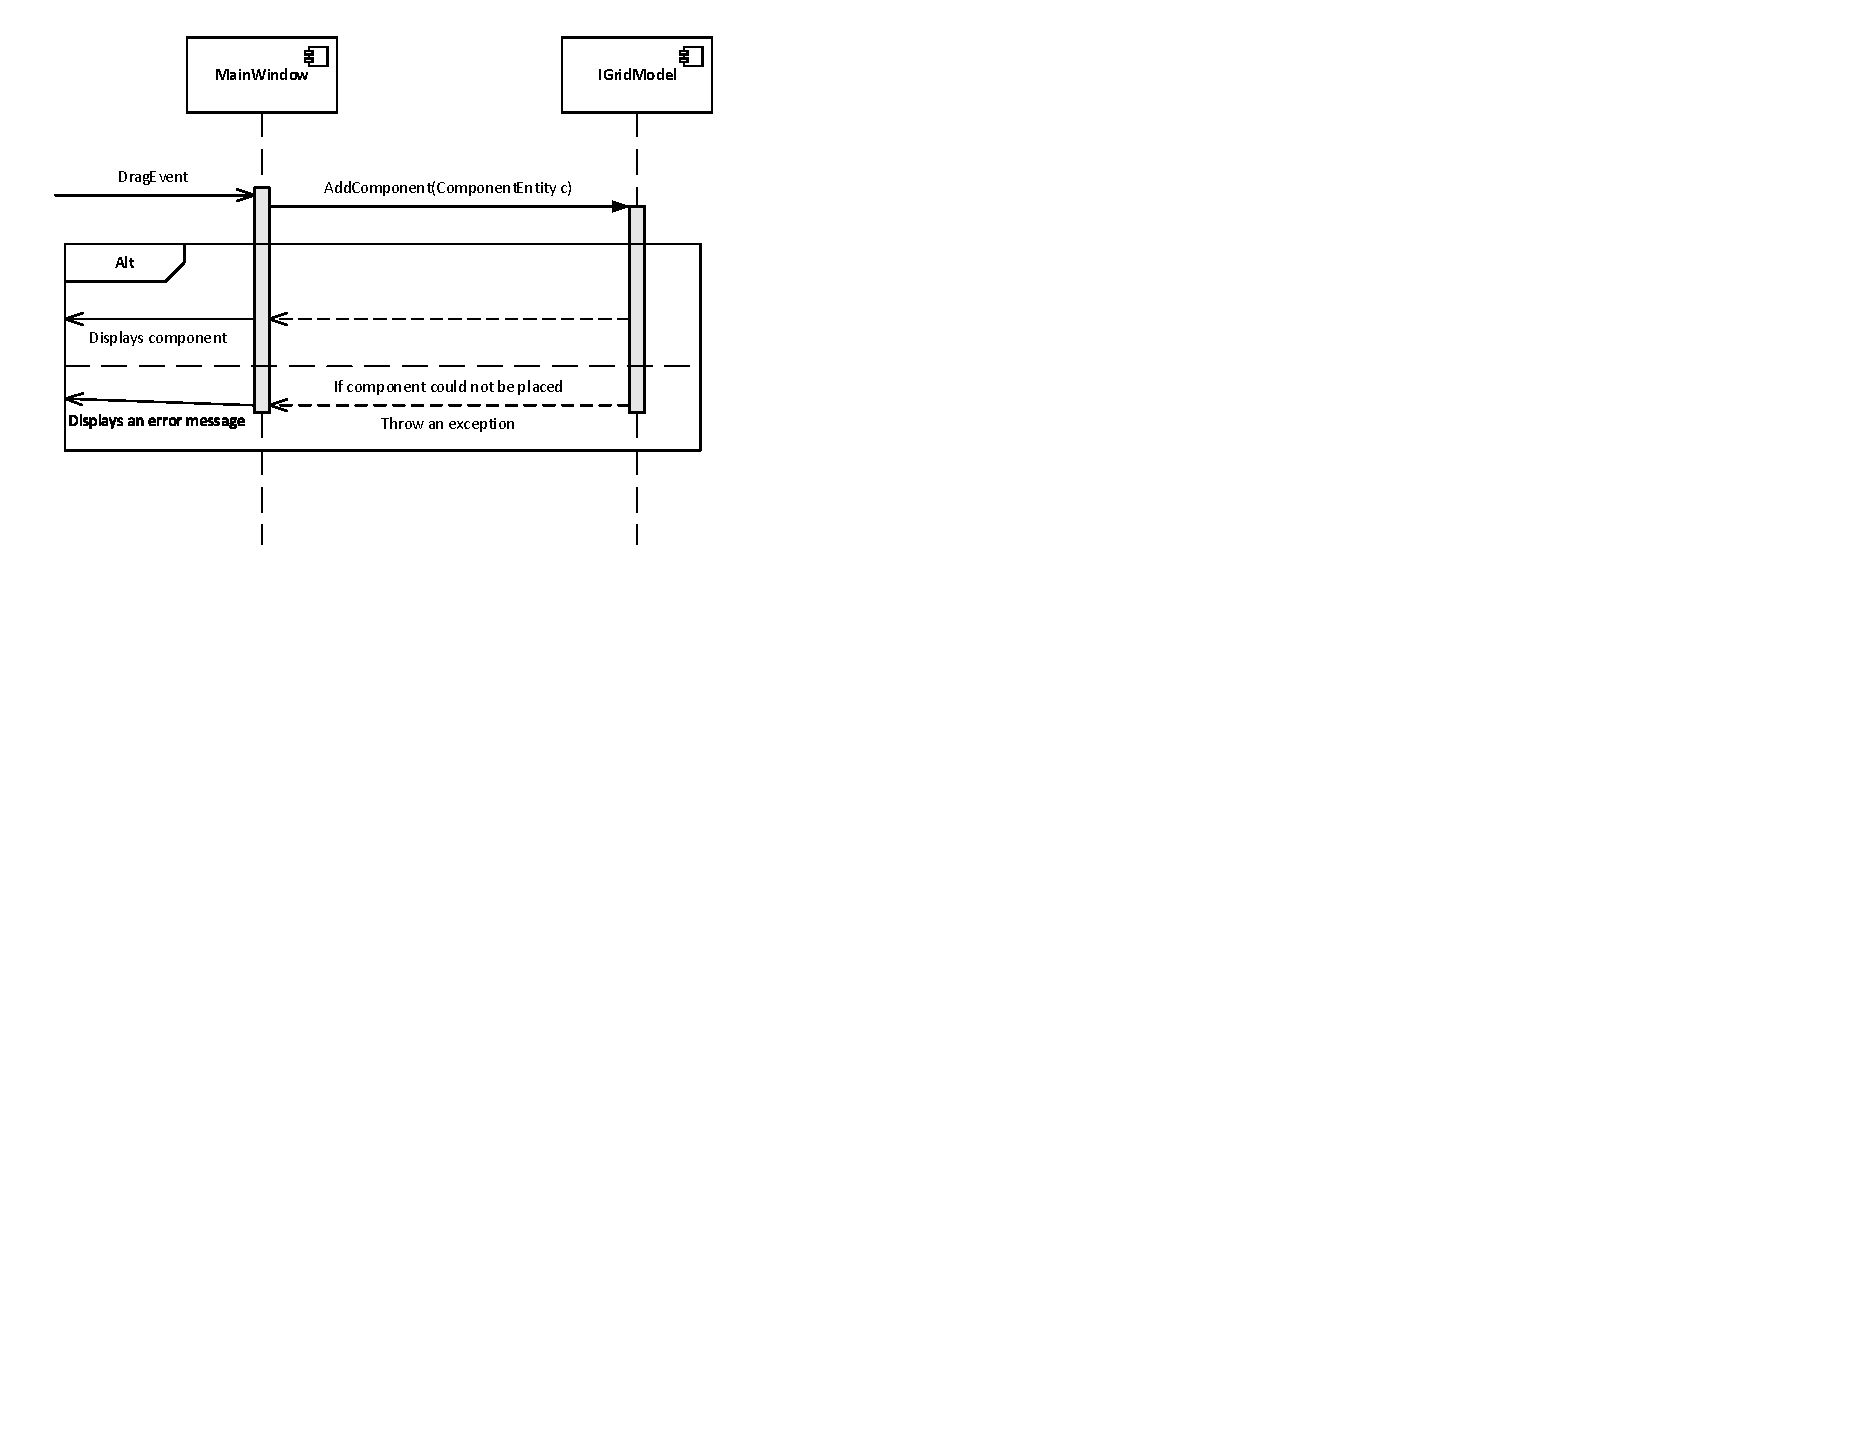
\includegraphics{figures/ConfigTrafficLight}
	\caption{Configuring traffic light times.}
\end{figure}

\begin{figure}[!ht]
	\centering
	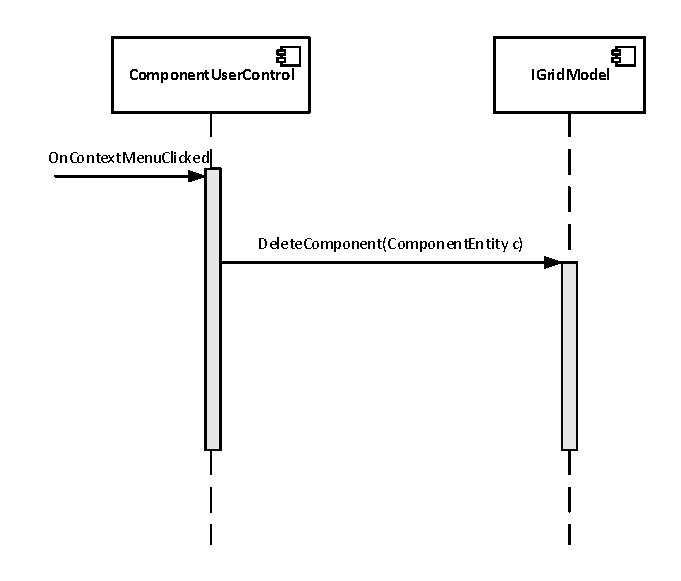
\includegraphics{figures/DeleteComponent}
	\caption{Deleting components.}
\end{figure}

\begin{figure}[!ht]
	\centering
	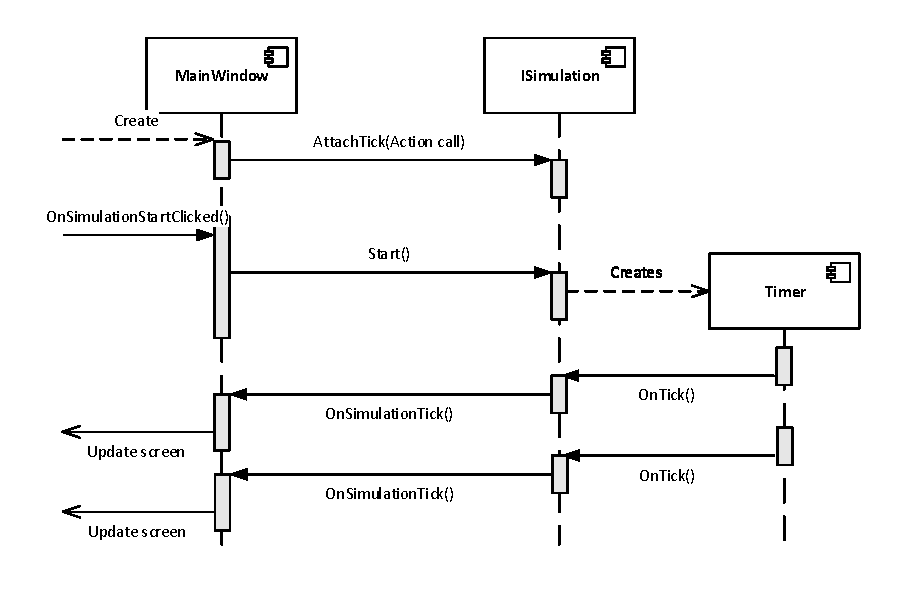
\includegraphics{figures/RunningSimulation}
	\caption{Running simulation.}
\end{figure}

\begin{figure}[!ht]
	\centering
	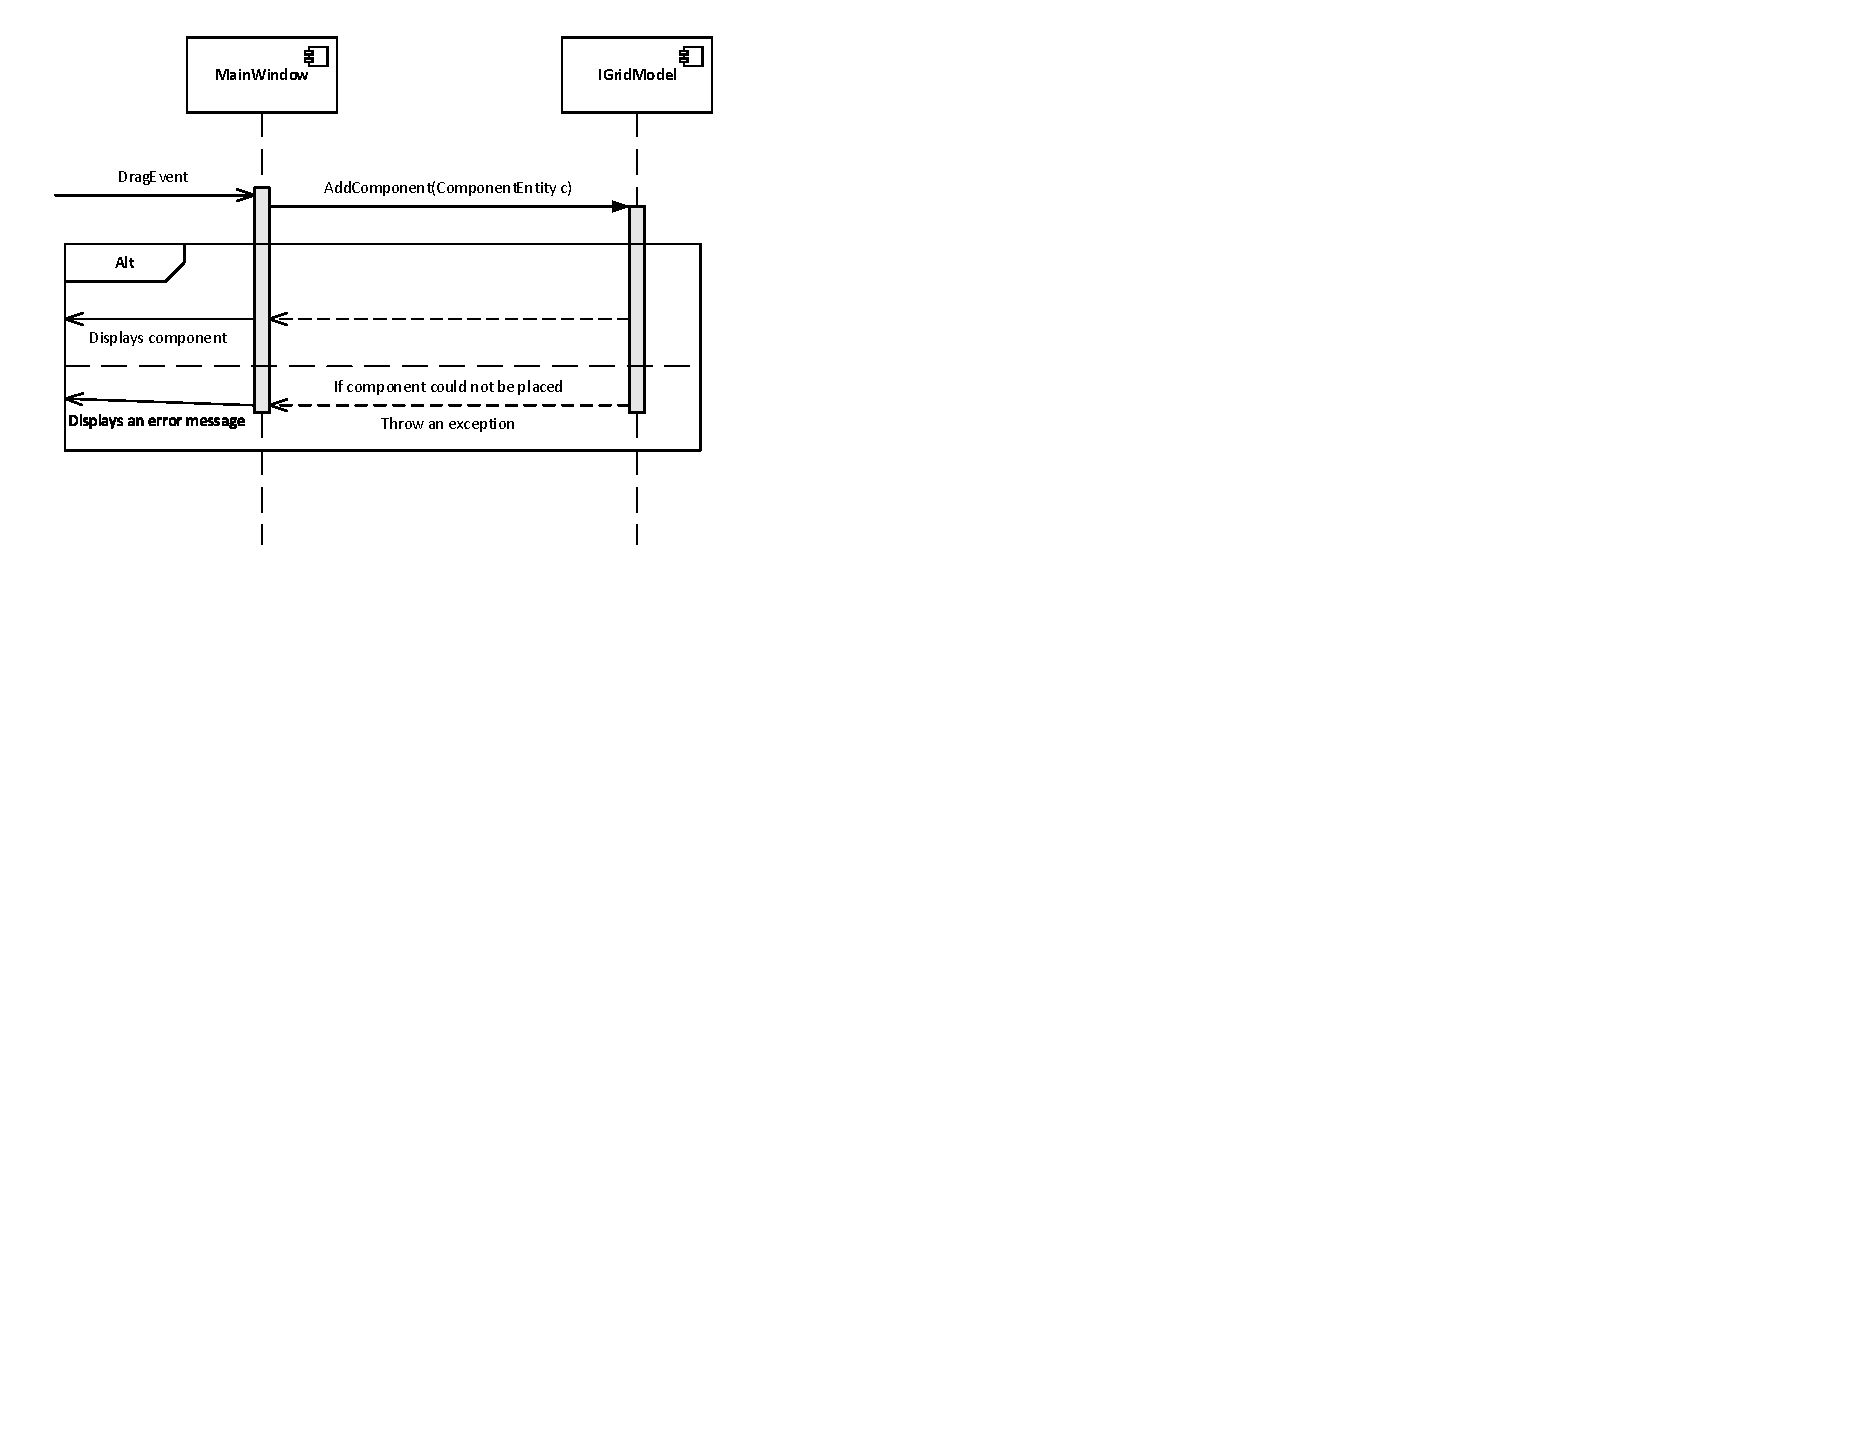
\includegraphics{figures/Stopping}
	\caption{Stopping simulation.}
\end{figure}

\begin{figure}[!ht]
	\centering
	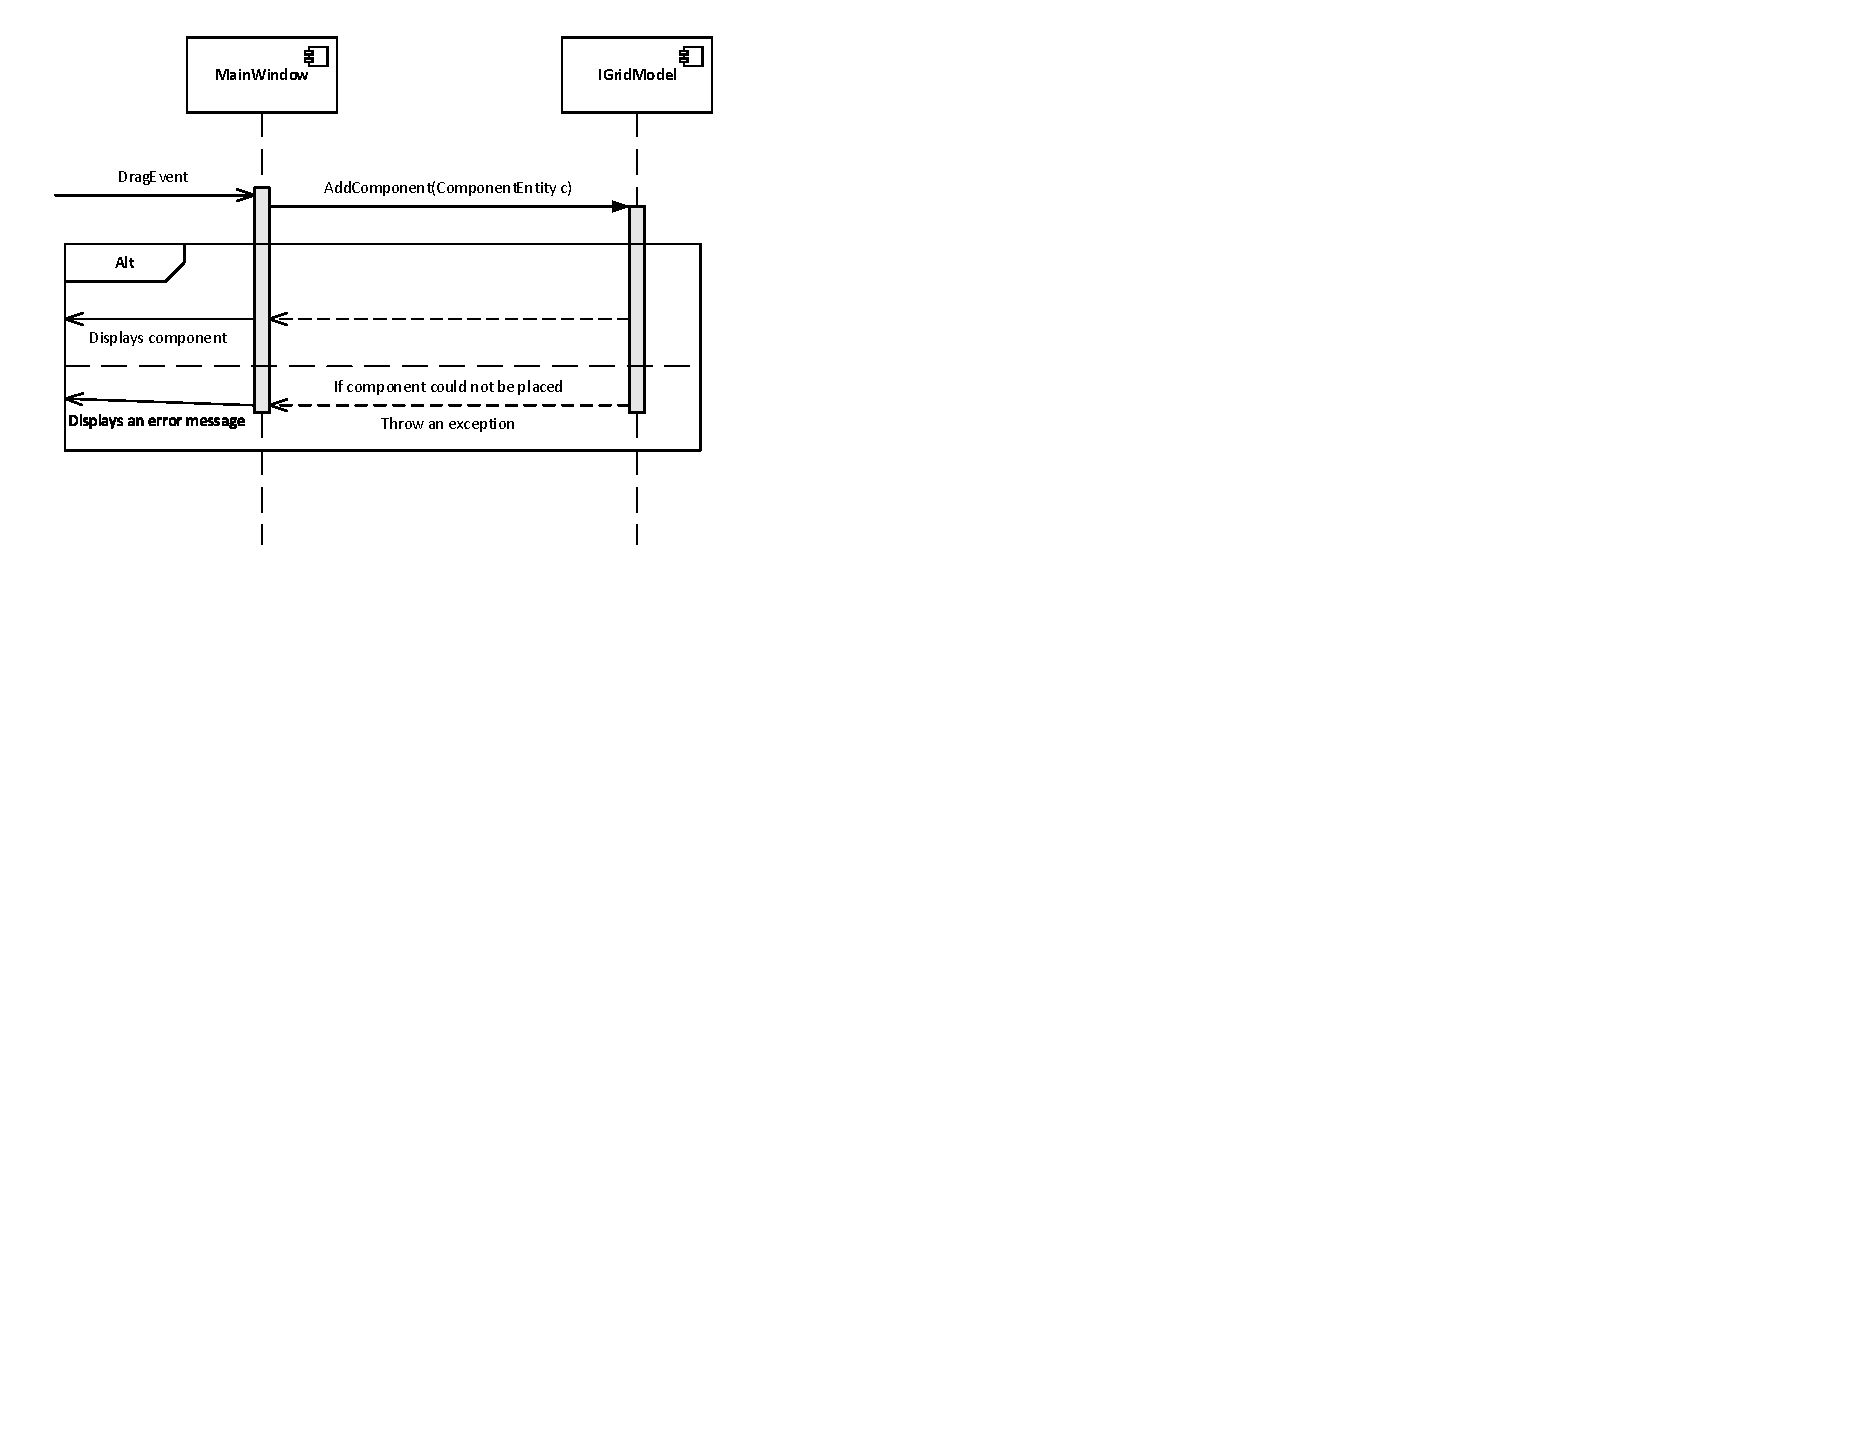
\includegraphics{figures/Pausing}
	\caption{Pausing simulation.}
\end{figure}

\begin{figure}[!ht]
	\centering
	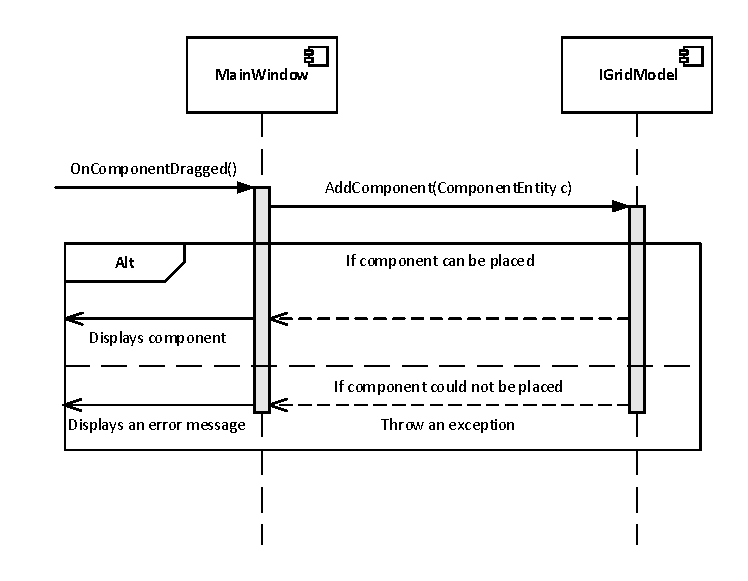
\includegraphics{figures/LoadFile}
	\caption{Opening a file.}
\end{figure}

\begin{figure}[!ht]
	\centering
	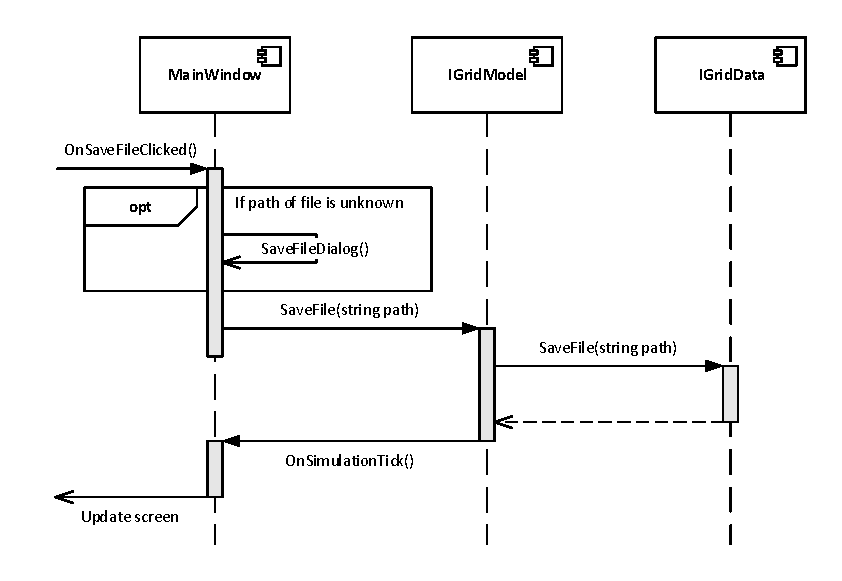
\includegraphics{figures/SaveFile}
	\caption{Saving a file.}
\end{figure}

\begin{figure}[!ht]
	\centering
	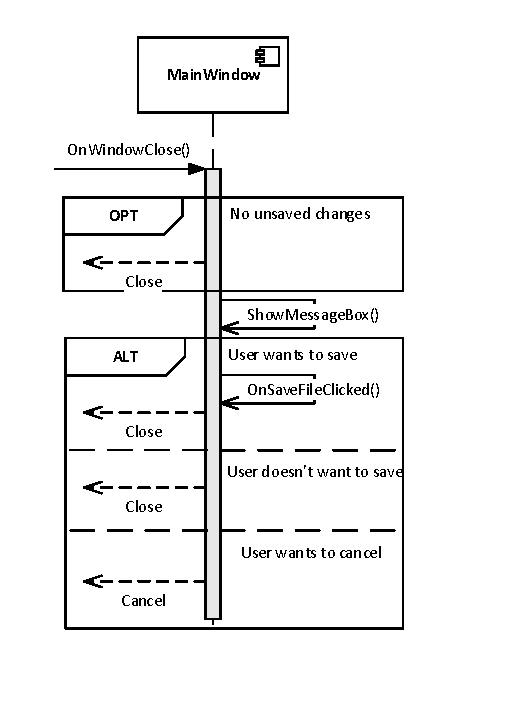
\includegraphics{figures/CloseWindow}
	\caption{Close window.}
\end{figure}